\fontsize{9}{10.5}\selectfont
\par\Needspace{100pt}\section*{Older Q2: Conceptual models, behaviour and process}\label{older-q2}
\phantomsection\addcontentsline{toc}{section}{Older Q2: Conceptual models, behaviour and process}
\markboth{Older papers | Q2}{}
\textbf{Shared method:} apply Chapters 4--5 to the named object/workflow; use \hyperref[answer-waterfall]{W, p.\ \pageref{answer-waterfall}} and \hyperref[answer-scrum]{S, p.\ \pageref{answer-scrum}} for process questions.
\par\Needspace{85pt}\subsection*{AY2022/23 S1: Car sales --- Q2 (25 marks)}\label{old-2223-s1-q2}

\sectionlabel{h-q2--analysis-and-process-25-marks}
\textbf{(a) Hold-car conceptual classes with boundary/\allowbreak{}control/\allowbreak{}entity stereotypes (8). (b) Dialog map for holding a car (8). (c) Can customer involvement fix Waterfall's response to changing requirements? (4). (d) Estimate Scrum progress and timely completion (5).}


\textbf{(a)} The external payment system is represented by a payment boundary, not an entity.




\par\smallskip\noindent\begin{minipage}{\linewidth}\centering
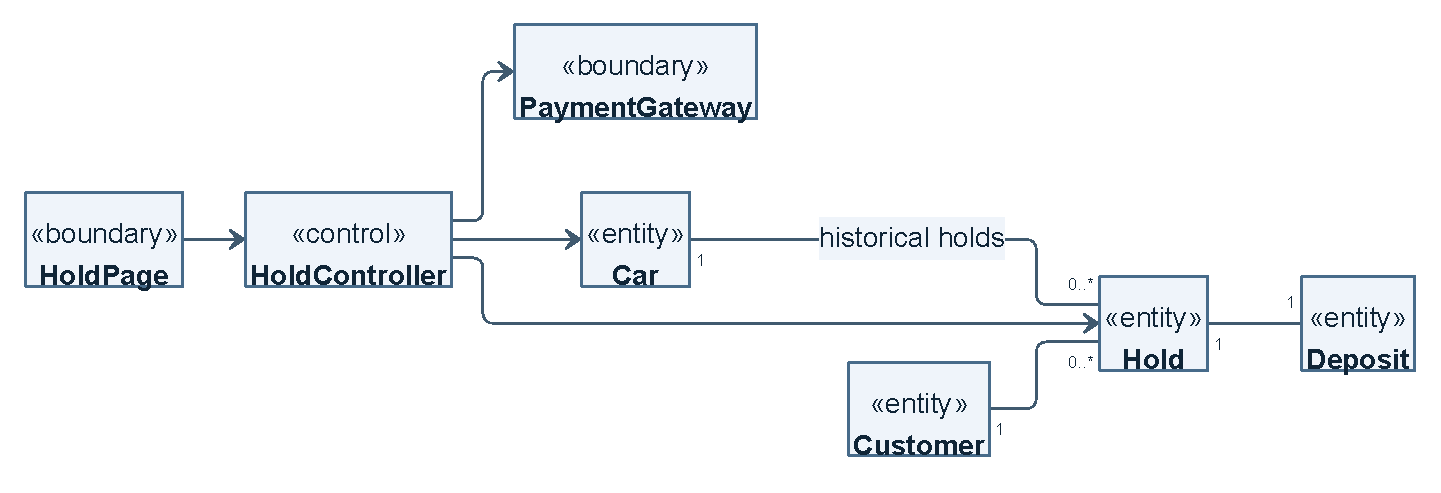
\includegraphics[width=405.68pt]{images/fig-049.pdf}
\captionof{figure}{Car sales: Q2 --- Analysis and process (25 marks)}\end{minipage}\par\smallskip



Constraint: each Car has \textbf{at most one active Hold}, even though historical holds are many. Customer may have multiple holds on different cars; Appendix A does not prohibit that. Attributes/\allowbreak{}operations are deliberately omitted for this analysis question.

\textbf{(b)} The hold dialog models screens, not physical car states.




\par\smallskip\noindent\begin{minipage}{\linewidth}\centering
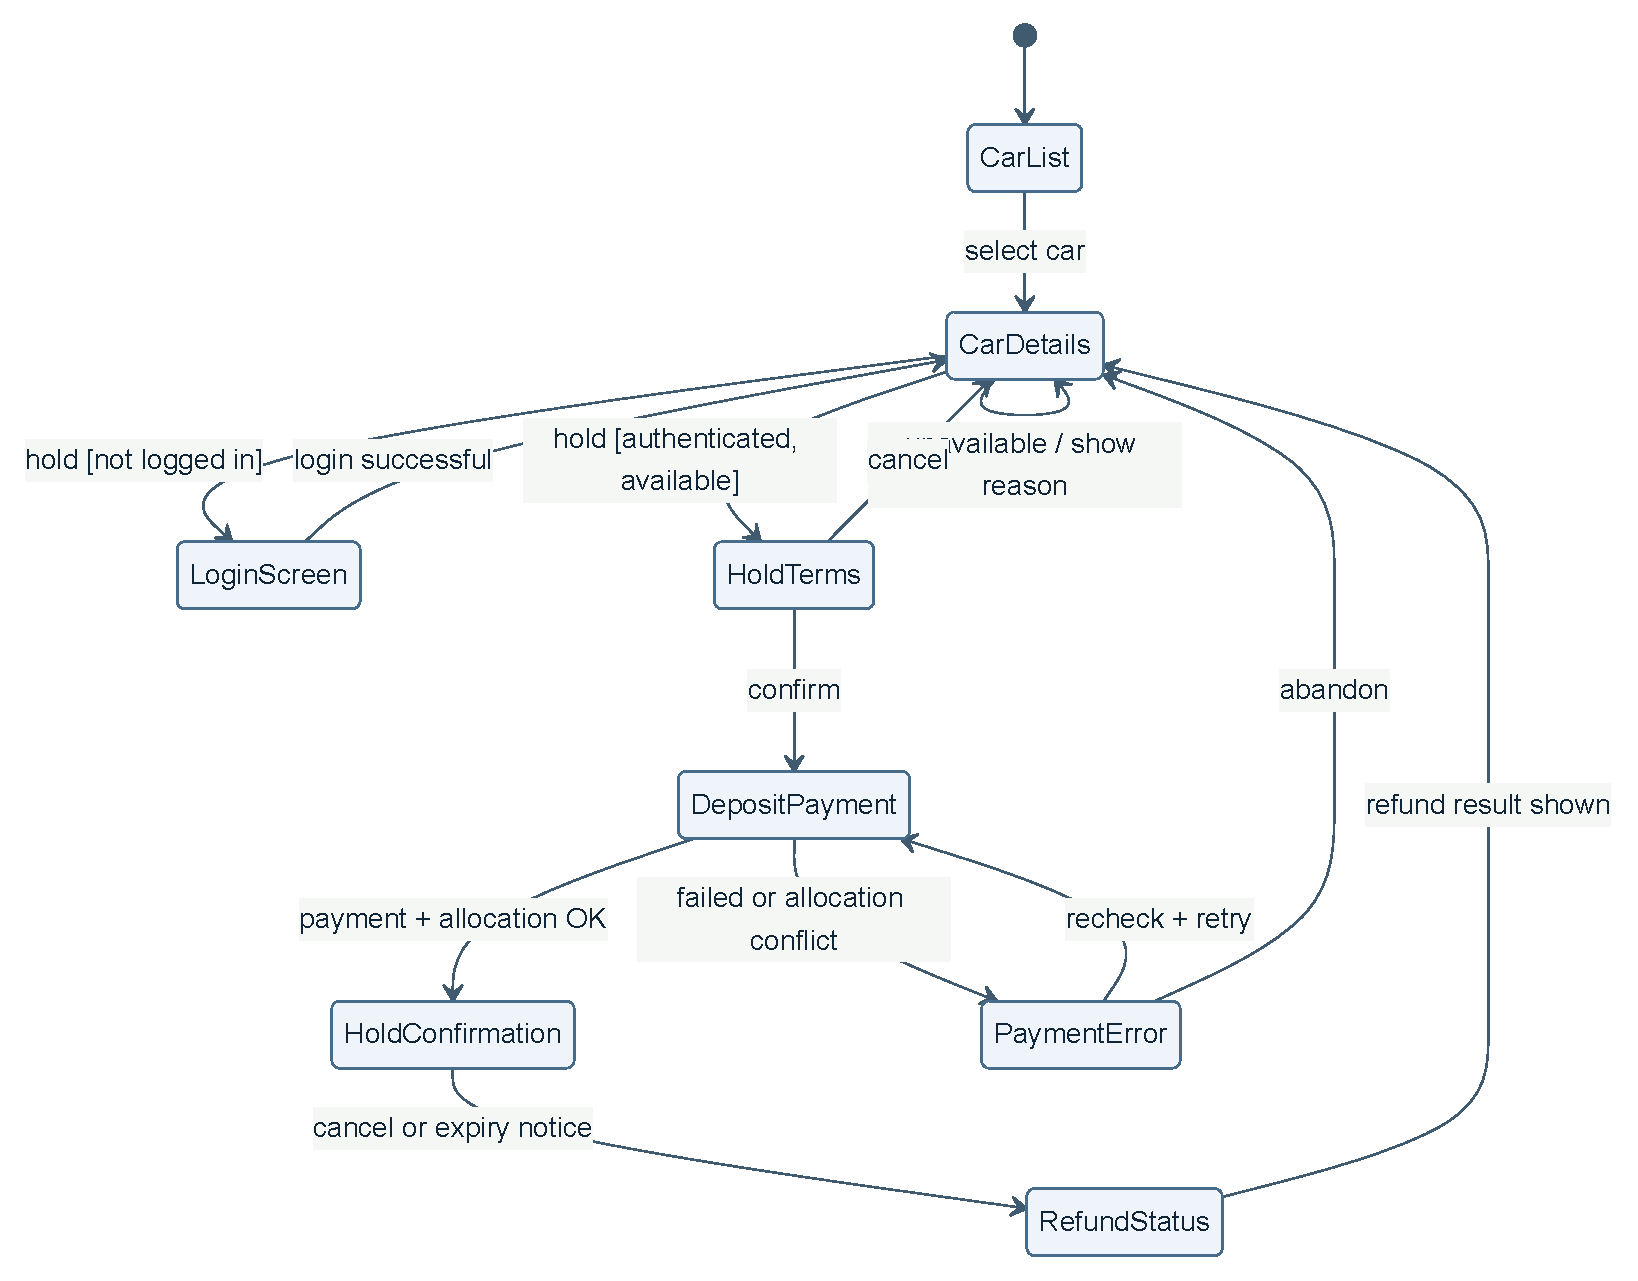
\includegraphics[width=461.12pt]{images/fig-050.pdf}
\captionof{figure}{Car sales: Q2 --- Analysis and process (25 marks)}\end{minipage}\par\smallskip



Terms/\allowbreak{}error/\allowbreak{}refund screens are proposed interface details. The business invariants from Q1 still apply.

\textbf{(c)} Use \hyperref[answer-waterfall]{W, p.\ \pageref{answer-waterfall}}: customer reviews expose change early; agreed downstream impact/replanning is still necessary.

\textbf{(d)} Use \hyperref[answer-scrum]{S, p.\ \pageref{answer-scrum}}: track remaining effort/velocity with a burndown; forecast capacity and negotiate priorities as scope changes.
\par\Needspace{85pt}\subsection*{AY2022/23 S2: Shopping chatbot --- Q2 (25 marks)}\label{old-2223-s2-q2}

\sectionlabel{h-q2--analysis-and-development-process-25-marks}
\textbf{(a) Replacement conceptual classes with stereotypes (7). (b) Replacement activity with user/\allowbreak{}chatbot/\allowbreak{}existing-system participants (8). (c) Why reuse-based integration/\allowbreak{}configuration can force requirement compromises, and mitigation (4). (d) Scrum Master response to a bug threatening sprint completion (6).}


\textbf{(a)}




\par\smallskip\noindent\begin{minipage}{\linewidth}\centering
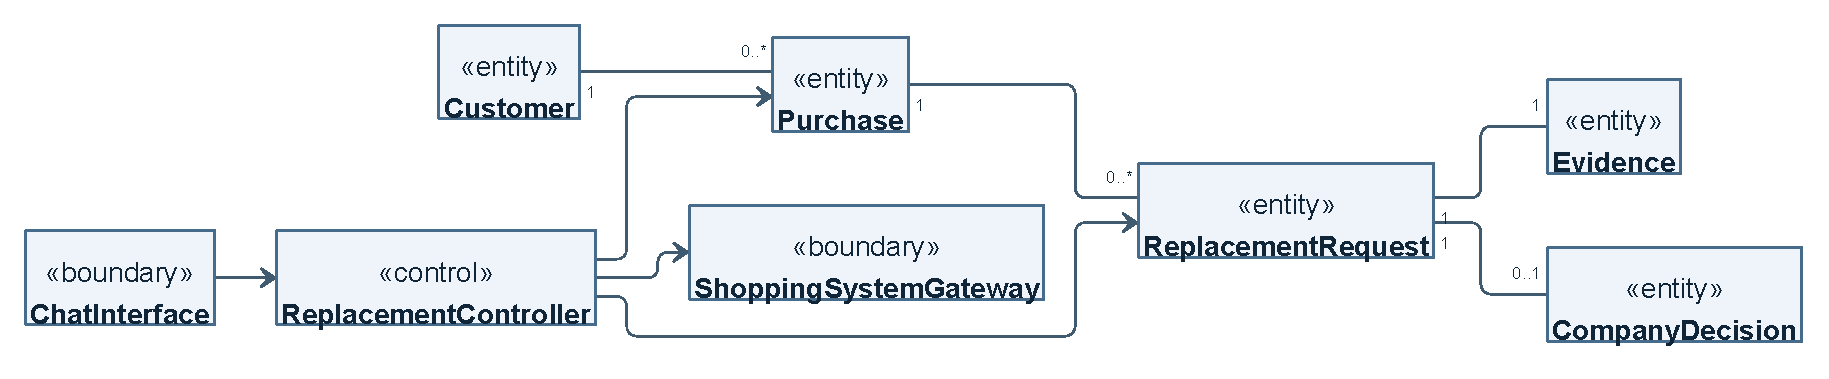
\includegraphics[width=514.00pt]{images/fig-054.pdf}
\captionof{figure}{Shopping chatbot: Q2 --- Analysis and development process (25 marks)}\end{minipage}\par\smallskip



Decision is absent while pending. Evidence groups photos, receipt and reason; its presence does not imply that an incomplete submission is approved.

\textbf{(b)} Subgraphs approximate activity swimlanes. Company approval is an activity of the existing system's organisation, not an autonomous chatbot decision.






\par\smallskip\noindent\begin{minipage}{\linewidth}\centering
{\scriptsize\textbf{Eligibility and evidence}}\par\smallskip
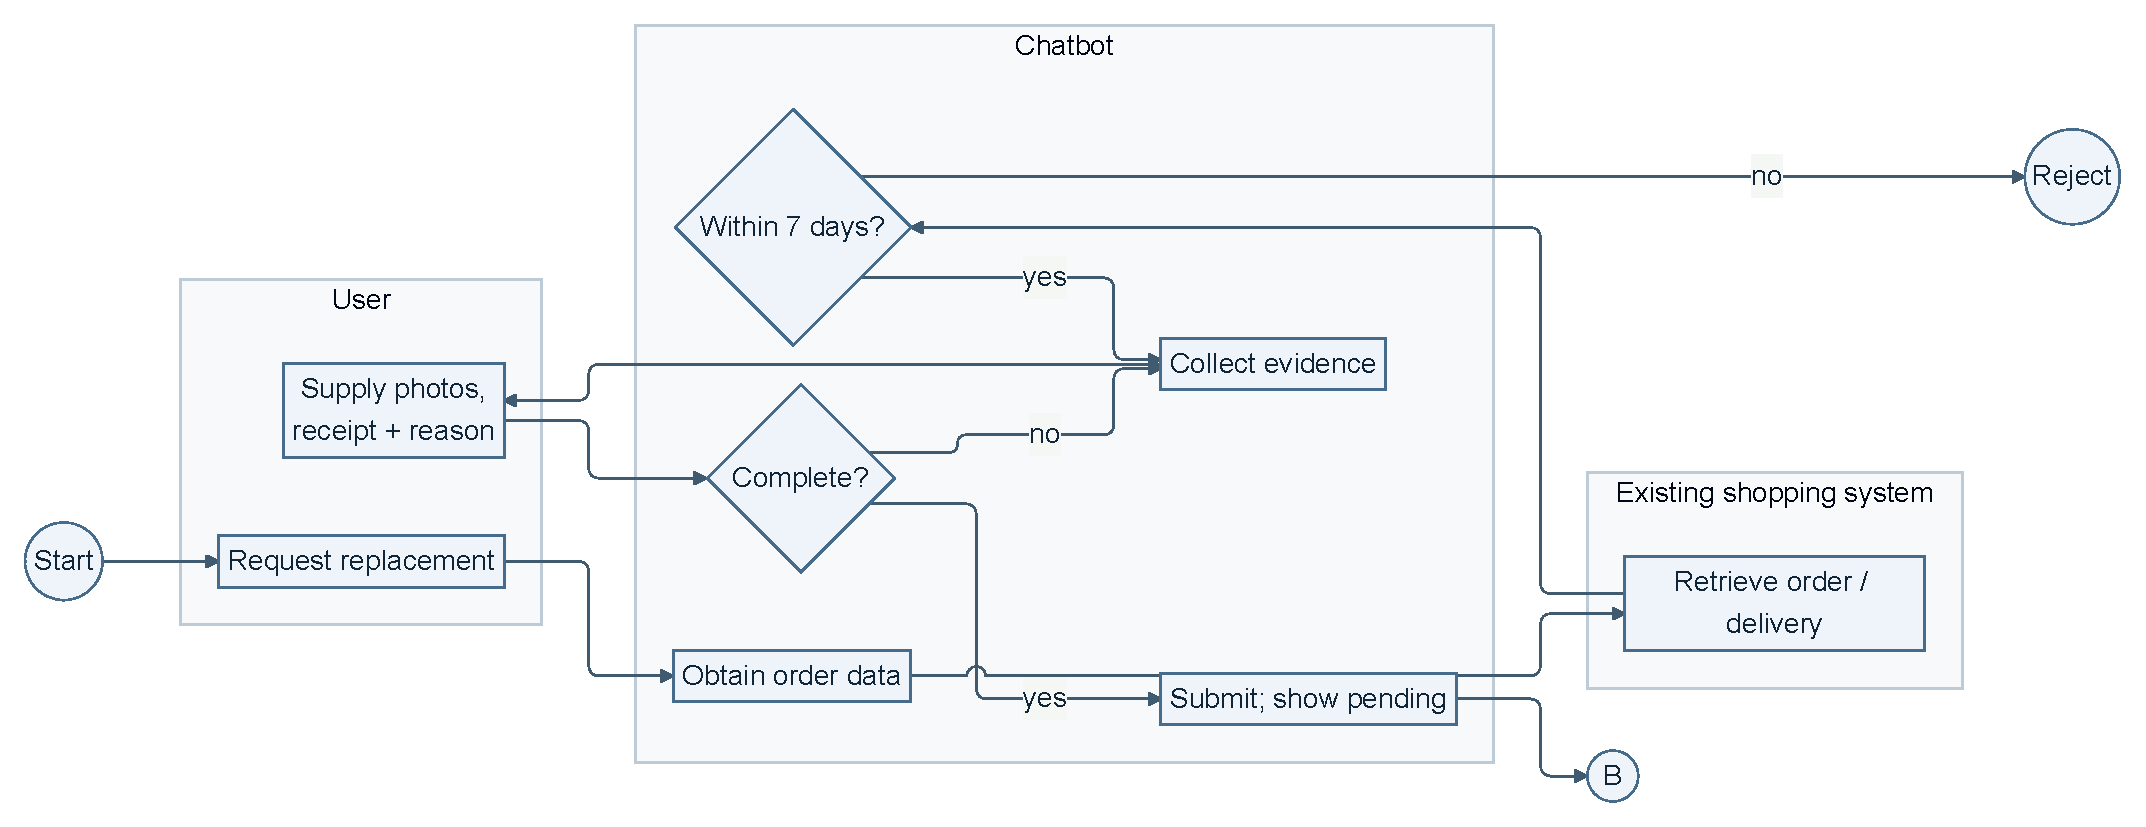
\includegraphics[width=514.00pt]{images/fig-055-a.pdf}\par\smallskip
{\scriptsize\textbf{Company decision and outcome}}\par\smallskip
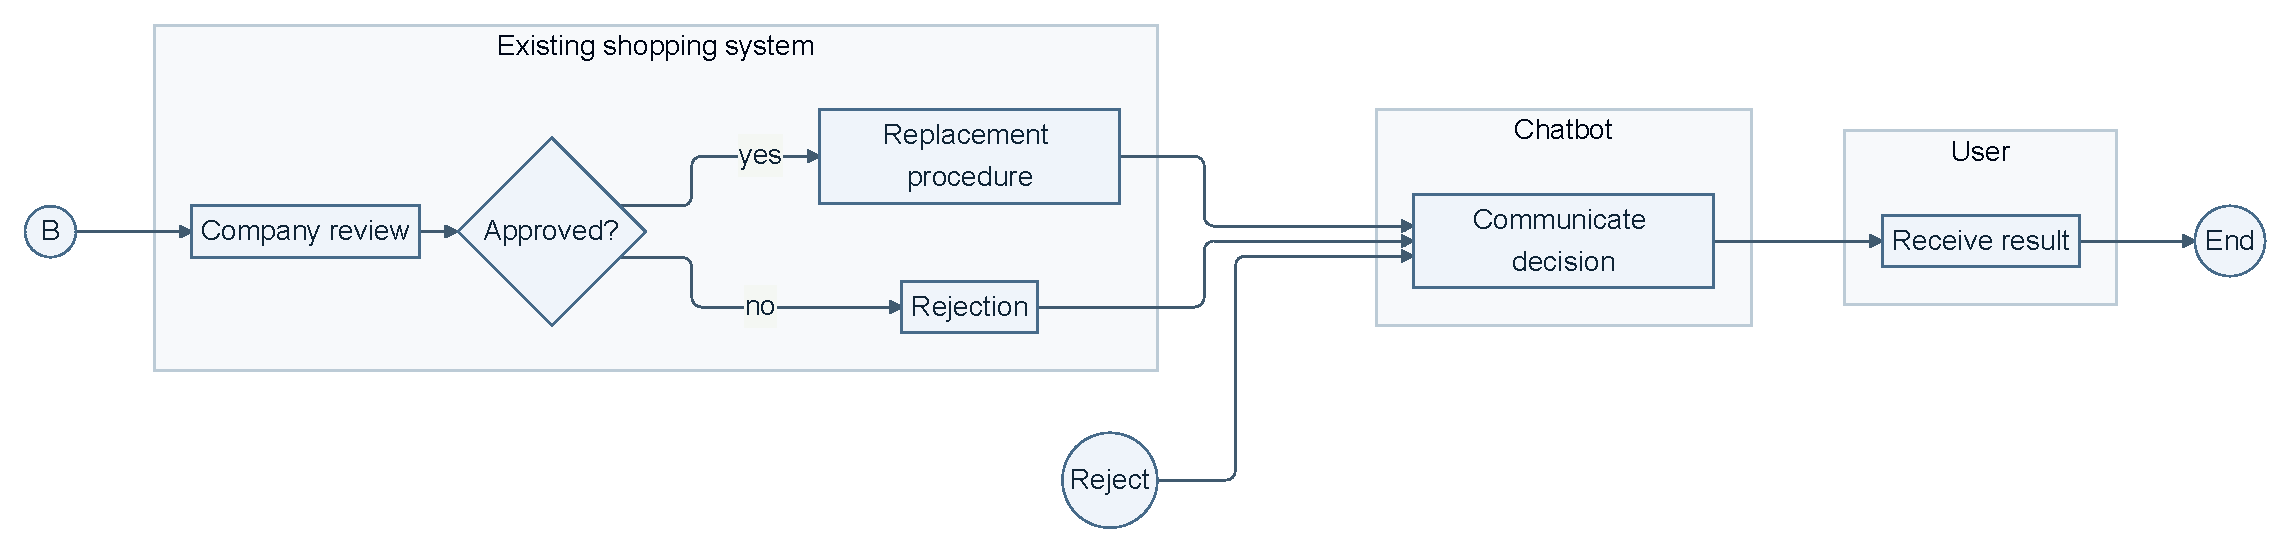
\includegraphics[width=514.00pt]{images/fig-055-b.pdf}\par\smallskip
\captionof{figure}{Shopping chatbot: Q2 --- Analysis and development process (25 marks)}\end{minipage}\par\smallskip









\textbf{(c)} Use \hyperref[answer-waterfall]{W, p.\ \pageref{answer-waterfall}} for reuse: compare the existing shop with must-have requirements, prototype its interfaces, negotiate acceptable compromises and adapt/build unmet essentials.

\textbf{(d)} Apply \hyperref[answer-scrum]{S, p.\ \pageref{answer-scrum}}: expose the bug, let developers investigate, assess Sprint Goal/severity, negotiate less essential work and review prevention. The Scrum Master facilitates.
\par\Needspace{85pt}\subsection*{AY2023/24 S1: DevSecOps --- Q2 (25 marks)}\label{old-2324-s1-q2}

\sectionlabel{h-q2--analysis-and-agile-25-marks}
\textbf{(a) Security-check conceptual classes/\allowbreak{}stereotypes (8). (b) Activity diagram with swimlanes (8). (c) Explain how incremental development can be plan-driven or agile (4). (d) Why may agile struggle with widely varying team skills? (5).}


\textbf{(a)}




\par\smallskip\noindent\begin{minipage}{\linewidth}\centering
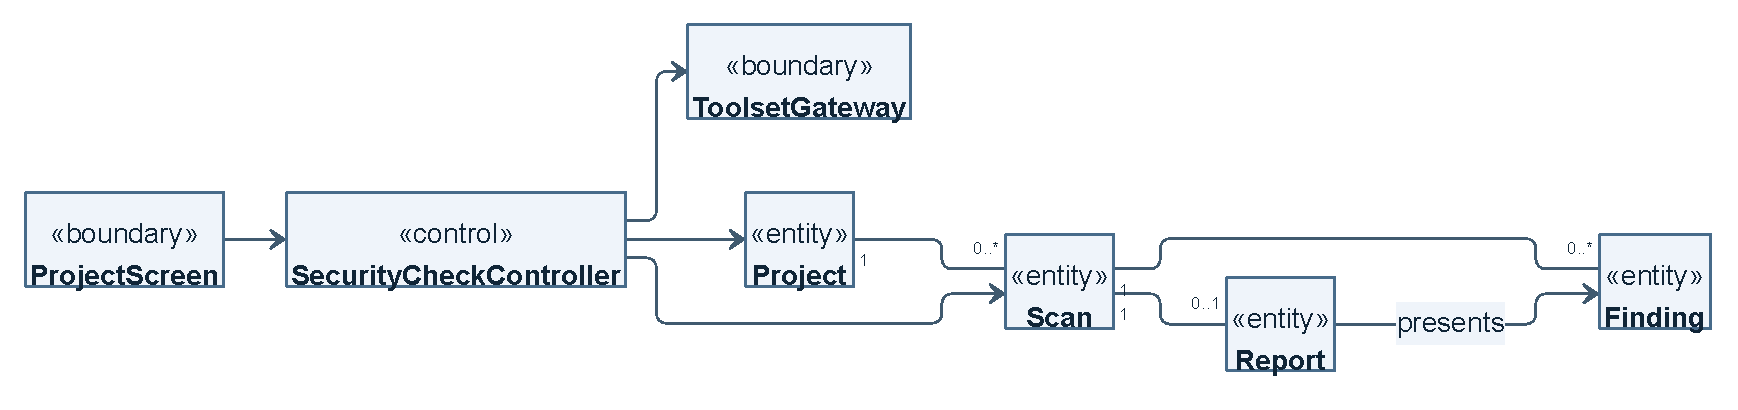
\includegraphics[width=488.84pt]{images/fig-059.pdf}
\captionof{figure}{DevSecOps: Q2 --- Analysis and agile (25 marks)}\end{minipage}\par\smallskip



\textbf{(b)} The external tool lane represents selected engines, not people inside the platform. Activities may be scheduled in parallel if dependencies permit; that scheduling is not specified by Appendix A.






\par\smallskip\noindent\begin{minipage}{\linewidth}\centering
{\scriptsize\textbf{A: scan and report}}\par\smallskip
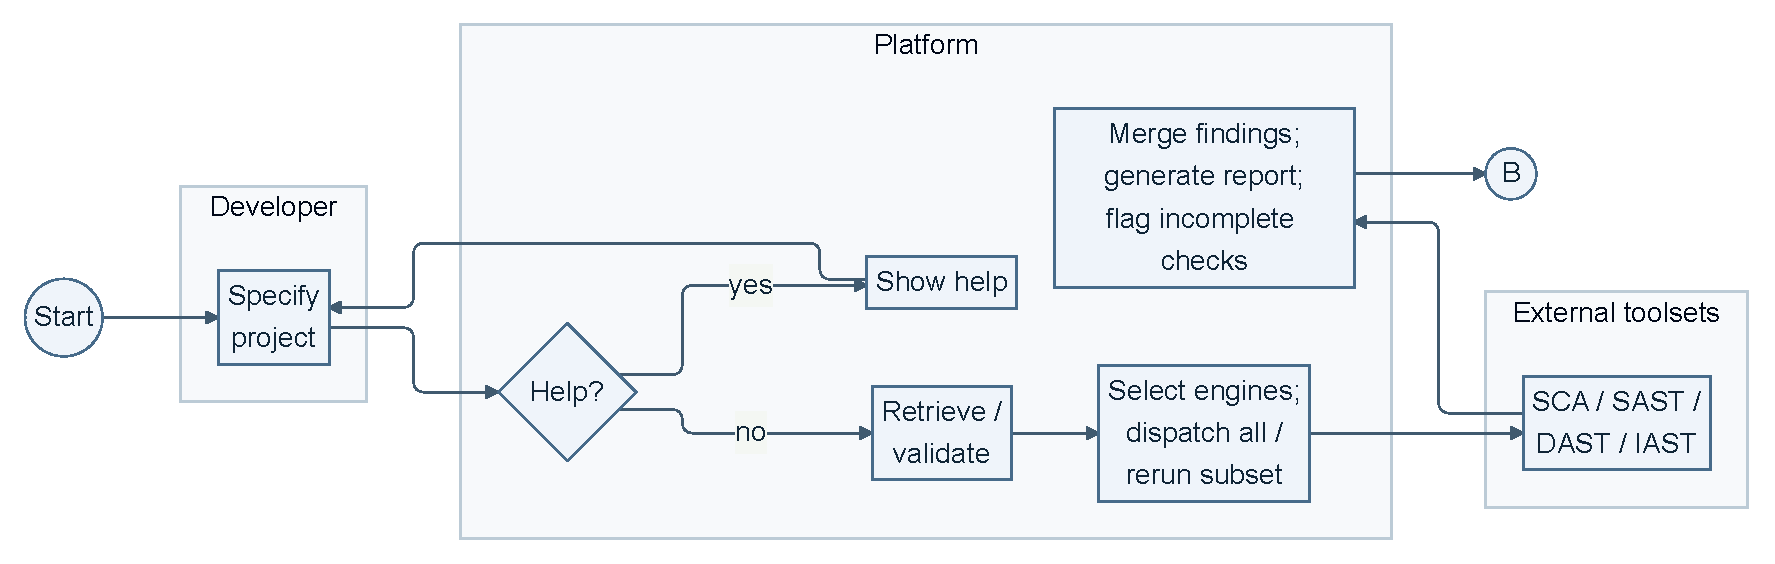
\includegraphics[width=454.00pt]{images/fig-060-a.pdf}\par\smallskip
{\scriptsize\textbf{B: review, mitigation and selected rerun}}\par\smallskip
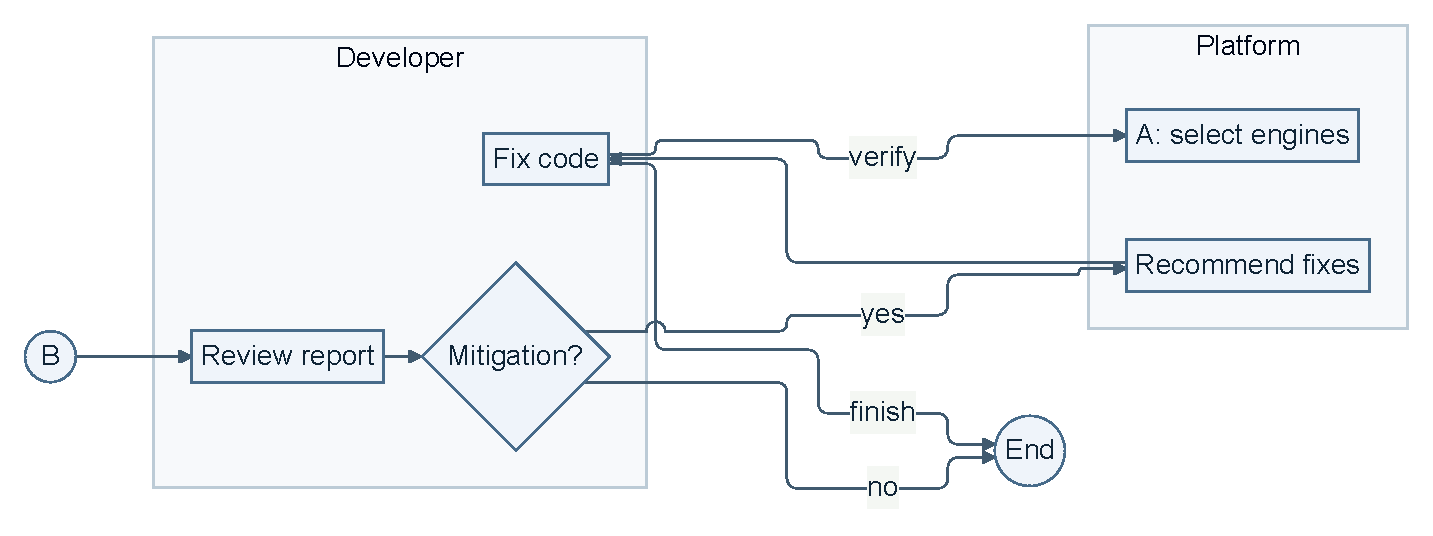
\includegraphics[width=366.80pt]{images/fig-060-b.pdf}\par\smallskip
\captionof{figure}{DevSecOps: DevSecOps activity workflow --- combined scan/report and review/rerun phases; B continues below, A returns to engine selection.}\end{minipage}\par\smallskip










\textbf{(c)} Use \hyperref[answer-waterfall]{W, p.\ \pageref{answer-waterfall}}: increments may be preplanned or reprioritised through feedback; delivery structure alone does not establish agile management.

\textbf{(d)} Use \hyperref[answer-scrum]{S, p.\ \pageref{answer-scrum}}: uneven skills risk quality, estimates, expert bottlenecks and integration. Pair/mentor, standardise and automate tests; diversity itself is not disqualifying.
\par\Needspace{85pt}\subsection*{AY2023/24 S2: CodeAgent --- Q2 (25 marks)}\label{old-2324-s2-q2}

\sectionlabel{h-q2--reviewer-analysis-qa-states-and-process-25-marks}
\textbf{(a) Reviewer conceptual classes/\allowbreak{}stereotypes (9). (b) QA-Checker state machine (7). (c) Two ways plan-driven projects can handle changing requirements (4). (d) Importance of Scrum velocity (5).}


\textbf{(a)}




\par\smallskip\noindent\begin{minipage}{\linewidth}\centering
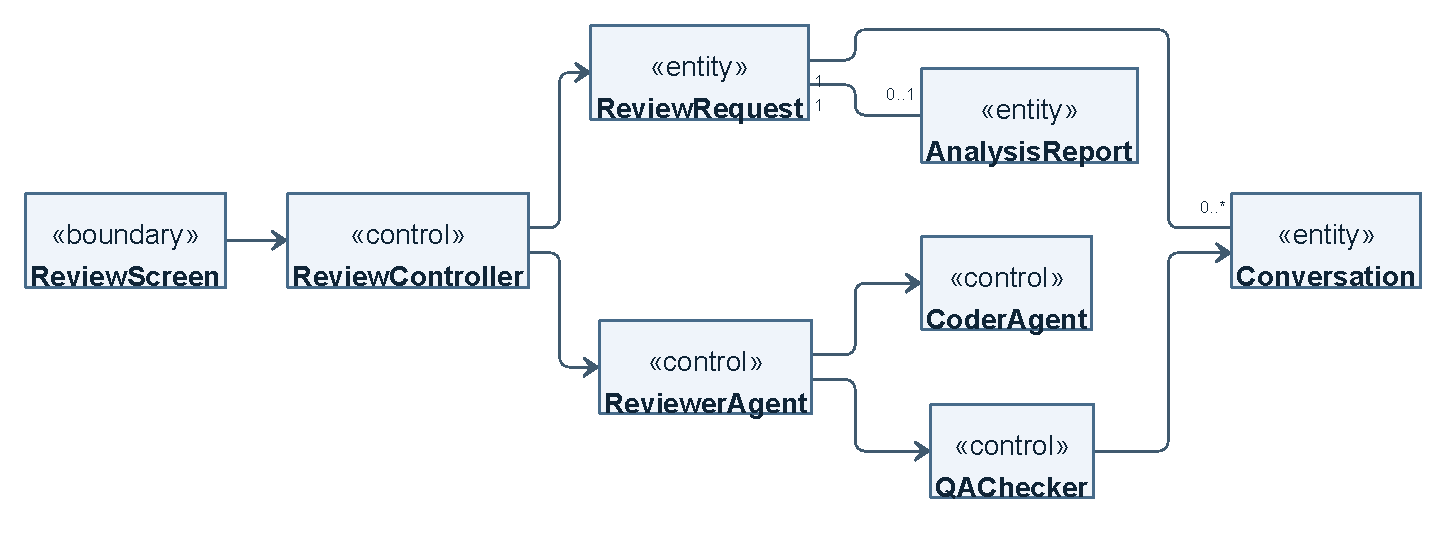
\includegraphics[width=407.44pt]{images/fig-065.pdf}
\captionof{figure}{CodeAgent: Q2 --- Reviewer analysis, QA states and process (25 marks)}\end{minipage}\par\smallskip



Agents coordinate behaviour; they are not merely stored domain records. ReviewRequest groups commit, message and original files. Report is absent before completion; unresolved status is possible.

\textbf{(b)} Let \code{n} count answers received and \code{max} be the configured maximum dialogue count. Assume \code{max \ensuremath{\geq} 1}. On the first received answer set \code{n=\allowbreak{}1}.




\par\smallskip\noindent\begin{minipage}{\linewidth}\centering
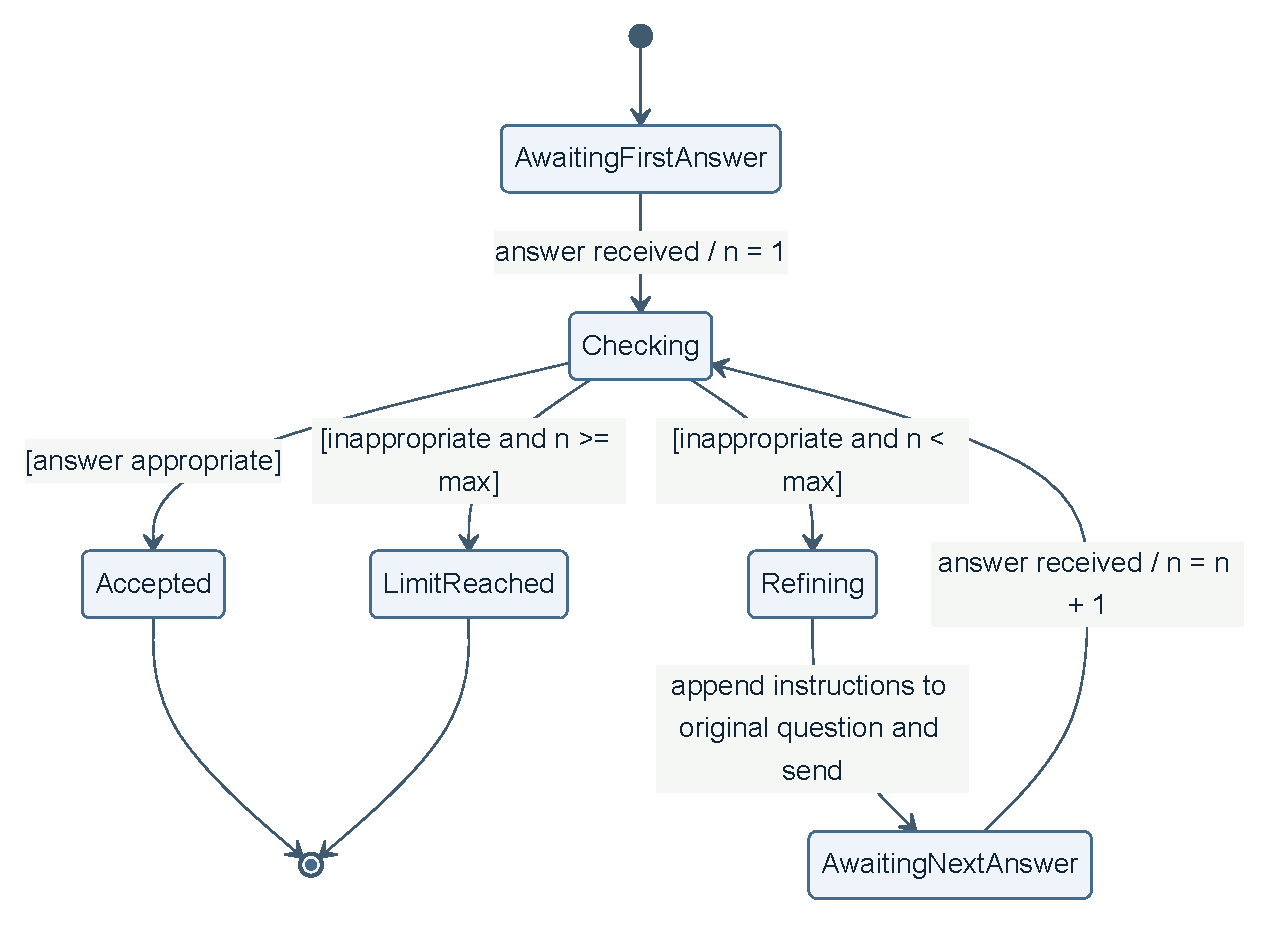
\includegraphics[width=357.72pt]{images/fig-066.pdf}
\captionof{figure}{CodeAgent: Q2 --- Reviewer analysis, QA states and process (25 marks)}\end{minipage}\par\smallskip

\begin{studycolumns}
\vspace{0pt}



Accept an appropriate answer even on the last permitted round. LimitReached means unresolved, not accepted. This models supervision of \textbf{one conversation}; a new conversation starts a new instance/\allowbreak{}reset.

\textbf{(c)} Apply \hyperref[answer-waterfall]{W, p.\ \pageref{answer-waterfall}} with two measures: early prototypes/reviews or planned increments; approved change control updating affected baselines, schedule, budget and tests.

\textbf{(d)} Use \hyperref[answer-scrum]{S, p.\ \pageref{answer-scrum}}: completed velocity supports feasible sprint selection and remaining-effort forecasts. Reforecast capacity; exclude unfinished work and inflated estimates.
\end{studycolumns}

